\begin{frame}
  \begin{block}{PEC 287/2016}
    \begin{itemize}
      \item \textbf{Ementa}
      \begin{itemize}
        \item Altera os arts. 37, 40, 109, 149, 167, 195, 201 e 203 da
        Constituição, para dispor sobre a seguridade social, estabelece regras
        de transição e dá outras providências
      \end{itemize}
      \item \textbf{Autor}
      \begin{itemize}
        \item Poder Executivo
      \end{itemize}
      \item \textbf{Situação}
      \begin{itemize}
        \item Pronta para Pauta no PLENÁRIO (PLEN)
      \end{itemize}
    \end{itemize}
  \end{block}
\end{frame}

\begin{frame}{Como é}
  \begin{figure}[h]
  	\begin{center}
      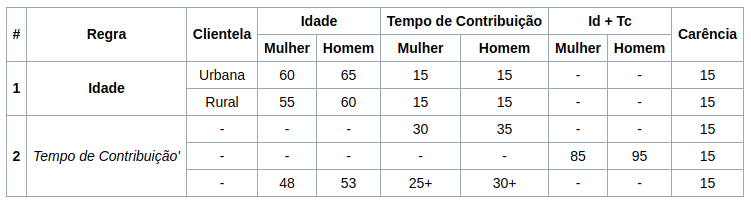
\includegraphics [scale=0.42]{./Figures/comoe}
     % \caption {Estimativa de dispositivos conectados à Internet.}
  		%\label{fig:arq-imuno}
  	\end{center}
  \end{figure}
  \textbf{Fator Previdenciário}
  	\begin{center}
    $f = \frac{Tc \times a}{Es} \times \left ( 1 + \frac{(Id + Tc \times
    0,31)}{100} \right )$
  	\end{center}
  \begin{itemize}
    \scriptsize
    \item $f$: Fator previdenciário
    \item $Tc$: Tempo de contribuição até o momento da aposentadoria
    \item $Id$: Idade no momento da aposentadoria
    \item $Es$: Expectativa de sobrevida no momento da aposentadoria
  \end{itemize}
\end{frame}

\begin{frame}{Como fica}
  Modalidade Única
  \begin{figure}[h]
  	\begin{center}
      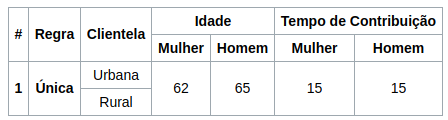
\includegraphics [scale=0.6]{./Figures/comofica}
     % \caption {Estimativa de dispositivos conectados à Internet.}
  		%\label{fig:arq-imuno}
  	\end{center}
  \end{figure}
\end{frame}

%\begin{frame}
%  \begin{block}{}
%    \begin{itemize}
%      \item
%    \end{itemize}
%  \end{block}
%\end{frame}

%\begin{frame}
%  \begin{block}{}
%  \end{block}
%\end{frame}

%\begin{frame}
%  \begin{figure}[h]
%  	\begin{center}
%      \includegraphics [scale=0.3]{./Figures/Device-Estimates}
%     % \caption {Estimativa de dispositivos conectados à Internet.}
%  		%\label{fig:arq-imuno}
%  	\end{center}
%  \end{figure}
%\end{frame}

%\begin{frame}{Redes de Acesso}
%	\begin{figure}[!htb]
%		\centering
%		\subfloat[DSL]{
%			\includegraphics[height=3.5cm]{./Figures/DSLaccess}
%			\label{figdroopy}}
%		\quad %espaco separador
%		\subfloat[Cable]{
%			\includegraphics[height=3.5cm]{./Figures/CableAccess}
%			\label{figsnoop}}
%		%\caption{Subfiguras}
%		%\label{fig01}
%	\end{figure}
%\end{frame}

%\begin{frame}[fragile]
%\scriptsize
%\begin{verbatim}
%\end{verbatim}
%\end{frame}

%\begin{frame}{\textit{Socket Programming with TCP}}
%\scriptsize
%\lstinputlisting[language=Python, caption={TCP Server.}]{./code/upperServer/TCPserver.py}
%\end{frame}

